\documentclass[12pt, a4paper,twoside]{tesi_upf}

%CODIFICATION
\usepackage[latin1]{inputenc}
%LENGUAGE
\usepackage[catalan,english]{babel}
%ONLY TO OBTAIN MARK BANK INDEX INDICATION A4
\usepackage[cam,a4,center,frame]{crop}
%INCLUDE GRAPHICS AND THE LOGO OF THE UPF
\usepackage{graphicx}
%FONTS TIMES OR GARAMOND, 
\usepackage{times}
%\usepackage{garamond}
%WITHOUT HEADINGS: NO MODIFICATION
\pagestyle{plain}
%FOR THE INDEX OF SUBJECTS
\usepackage{makeidx}
\makeindex
%BIBLIOGRAPHY STYLE
\bibliographystyle{unsrt}
%SELECT LANGUAGE
\selectlanguage{catalan}
 
\usepackage{cite}
% Equations
\usepackage{amsmath,amssymb,amsfonts}

% Hyperreferences
\usepackage{url}
%\usepackage{hyperref}


\usepackage{graphicx} 	  %% The graphicx package provides the includegraphics command.
\usepackage{amssymb} 	%% The amssymb package provides various useful mathematical symbols

\usepackage{color}
\usepackage{amsmath}
\usepackage{mathtools}
\usepackage{fullpage}
\usepackage{algorithmic}
\DeclareMathOperator*{\argmin}{argmin}
\DeclareMathOperator*{\argmax}{argmax}
\algsetup{linenosize=\small}
\usepackage[table,xcdraw]{xcolor}
\usepackage{multirow}
\usepackage[super]{nth}
\usepackage{graphicx,adjustbox}
\usepackage{comment}
\usepackage{setspace}
\usepackage{textcomp}
\usepackage{xspace}
\usepackage{siunitx}
\usepackage{epsfig}
\usepackage{epstopdf}
\usepackage{soul}
\usepackage{tablefootnote}
\DeclareMathOperator{\E}{\mathbb{E}} % Expectation Symbol
\usepackage[linesnumbered,ruled]{algorithm2e}
\usepackage{booktabs}
\usepackage[normalem]{ulem}
\usepackage{footnote}
\usepackage[misc,geometry]{ifsym} 
\bibliographystyle{abbrvnat}
\makesavenoteenv{tabular}

\usepackage[edges]{forest}
\usetikzlibrary{shadows,arrows.meta}

%Defining the styles used in trees
%Note that the fill colour is not defined here.
\tikzset{parent/.style={align=center,text width=2cm,rounded corners=2pt},
	child/.style={align=center,text width=5.5cm,rounded corners=6pt},
	grandchild/.style={text width=8cm}
}


\hyphenation{Re-use}

%THE TABLE OF CONTENTS IS TITLE CONTENTS
%\addto\captionscatalan
\renewcommand{\contentsname}{\Large \sffamily Table of contents}

%ADD YOUR DATA
\title{Enabling Spatial Reuse in Future Wireless Local Area Networks:\\ a Machine Learning \& Game Theoretic Proposal}
%\subtitle{The subtitle of the thesis: Required}
\author{Francesc Wilhelmi Roca}
\thyear{2020}
\department{of Information and Communication Technologies}
\supervisor{Boris Bellalta, Cristina Cano \& Anders Jonsson}

\begin{document}

\frontmatter
\maketitle
\cleardoublepage

%%%%%% Dedication
\noindent Write here your dedication
\cleardoublepage
%%%%%% End dedication

%%%%%% Thanks
\noindent {\Large \sffamily Acknowledgments} 
\cleardoublepage
%%%%%% End of thanks

%ABSTRACT IN TWO LEGUAGES.
\selectlanguage{english}
\section*{\Large \sffamily Abstract}
The Spatial Reuse (SR) operation is gaining momentum in the newest IEEE 802.11 family of standards due to the overwhelming requirements posed by next-generation wireless networks. In particular, the increasing traffic capacity and number of concurrent devices compromise the efficiency of Wireless Local Area Networks (WLANs) and throw into question their decentralized nature. The SR operation, initially introduced by the IEEE 802.11ax-2020/21 amendment and further studied in IEEE 802.11be-2024, is aimed at increasing the number of concurrent transmissions in an Overlapping Basic Service Set (OBSS), thus improving spectral efficiency. 

The SR operation has been initially defined as a distributed mechanism, but it is evolving towards coordinated schemes. Nevertheless, coordination entails communication and synchronization procedures that have not been defined yet. The necessary overhead to carry out coordination has implications on the performance of WLANs and remains unknown. Moreover, the coordinated scheme is not compatible with IEEE 802.11 devices not implementing it.

Given the SR-related problems faced by future WLAN deployments, Artificial Intelligence (AI) emerges as a promising solution able to overcome the challenges arisen from the complex and varying spatial interactions among devices. In particular, due to the challenges posed by coordination, in this thesis, we study the feasibility of Reinforcement Learning (RL)-based methods to overcome the SR problem in a decentralized manner.

... \textcolor{red}{[TO BE COMPLETED]}

\pagebreak
\selectlanguage{english}
\vspace*{\fill}
\section*{\Large \sffamily  Resum}

\vspace*{\fill}

\cleardoublepage
%END OF ABSTRACT

\section*{\Large \sffamily List of Publications}

\begin{enumerate}
	\item Wilhelmi, F., Mu�oz, S. B., Cano, C., Selinis, I., \& Bellalta, B. (2019). \textit{Spatial Reuse in IEEE 802.11 ax WLANs.} arXiv preprint arXiv:1907.04141.
	\item Wilhelmi, F., Barrachina-Mu�oz, S., \& Bellalta, B. (2019, October). \textit{On the Performance of the Spatial Reuse Operation in IEEE 802.11 ax WLANs.} In 2019 IEEE Conference on Standards for Communications and Networking (CSCN) (pp. 1-6). IEEE.
	\item Wilhelmi, F., Bellalta, B., Cano, C., \& Jonsson, A. (2017, October). \textit{Implications of decentralized Q-learning resource allocation in wireless networks}. In 2017 ieee 28th annual international symposium on personal, indoor, and mobile radio communications (pimrc) (pp. 1-5). IEEE.
	\item Wilhelmi, F., Cano, C., Neu, G., Bellalta, B., Jonsson, A., \& Barrachina-Mu�oz, S. (2019). \textit{Collaborative spatial reuse in wireless networks via selfish multi-armed bandits.} Ad Hoc Networks, 88, 129-141.
	\item Wilhelmi Roca, F., Barrachina Mu�oz, S., Bellalta, B., Cano Sand�n, C., Jonsson, A., \& Neu, G. (2019). \textit{Potential and pitfalls of multi-armed bandits for decentralized spatial reuse in WLANs.} Journal of Network and Computer Applications, 2019, 127.
	\item Barrachina-Mu�oz, S., Wilhelmi, F., Selinis, I., \& Bellalta, B. (2019, April). \textit{Komondor: a wireless network simulator for next-generation high-density WLANs.} In 2019 Wireless Days (WD) (pp. 1-8). IEEE.
	\item Wilhelmi, F., Barrachina-Munoz, S., Bellalta, B., Cano, C., Jonsson, A., \& Ram, V. (2020). \textit{A Flexible Machine-Learning-Aware Architecture for Future WLANs. IEEE Communications Magazine, 58(3), 25-31.}	
	\item Wilhelmi, F., Carrascosa, M., Cano, C., Ram, V., \& Bellalta, B. (2020). \textit{Usage of Network Simulators in Machine-Learning-Assisted 5G/6G Networks.}
\end{enumerate}
%Decentralized learning with cost in IEEE 802.11 WLANs
%Survey MABs for communications

%%PREFACE. 
%{\bf Preface}

\cleardoublepage
%END OF PREFACE

%TABLE OF CONTENTS: REQUIRED
\tableofcontents

%lIST OF FIGURES; ONLY IF THERE ARE FIGURES
%\listoffigures
%TO APPER THE LIST OF FIGURES IN THE TABLE OF CONTENTS 
%\addcontentsline{toc}{chapter}{List of figures}

%LIST OF TABLES; ONLY IF THERE ARE TABLES
%\listoftables
%TO APPEAR THE LIST OF TABLES IN THE TABLE OF CONTENTS
%\addcontentsline{toc}{chapter}{List of tables}

%START THE TEXT
\mainmatter

%%%%%%%%%%%%%%%%%
% INTRODUCTION
%%%%%%%%%%%%%%%%%
\chapter{Introduction}

% Introduction to IEEE 802.11 WLANs 
The Institute of Electrical and Electronics Engineers (IEEE) 802.11 family of protocols for wireless local area networks (WLANs) was first released in 1997 as a novel solution for physical (PHY) and medium access control (MAC) layers. Since that date, the standard has evolved to sustain the increasingly user requirements in terms of capacity, load, and coverage, as well as to serve for different purposes (e.g., mesh networking, security-enhanced communications, channel measurement, etc.). The set of novel and improved capabilities have been captured along the time in the plethora of amendments that followed the initial 802.11-1997 standard (e.g., 802.11b, 802.11g, 802.11h, etc.). 

% Next-generation of IEEE 802.11 WLAN standards
Looking forward, the next generation of WLAN standards is expected to revolutionize the telecommunications and converge along with 5G systems and beyond to expand to multiple domains, such as light communications (IEEE 802.11bb), Internet of Things (IEEE 802.11ah), vehicle-to-everything (IEEE 802.11bd), or next-generation positioning (IEEE 802.11az).%, or next-generation 60 GHz (IEEE 802.11ay).

One of the most influential amendments is the IEEE 802.11ax-2021 (11ax) amendment for High Efficiency (HE) WLANs \cite{bellalta2016ieee, deng2014ieee, khorov2018tutorial}, which primary goal is to enhance network efficiency in ultra-dense deployments, thus providing high capacity (up to 10 Gbps). The 11ax (commercially known as WiFi 6) includes a set of unprecedented techniques, such as Orthogonal Frequency Division Multiple Access (OFDMA), Downlink/Uplink Multi-User Multiple-Input-Multiple-Output (DL/UL MU-MIMO), and Spatial Reuse (SR), to address the broad range of issues arisen from high-density scenarios \cite{merlin2015tgax}.

% What is SR and what it is aimed to solve
This thesis focuses on the SR operation that was initially conceived for IEEE 802.11ax WLANs and that is now evolving in the IEEE 802.11be. SR is meant to enhance spectral efficiency by increasing the number of parallel transmissions in high-dense deployments. To this end, SR proposes a mechanism to improve the probability of ignoring transmissions which source is a device belonging to a different Basic Service Sets (aka inter-BSS transmissions). This can be done by applying a less restrictive carrier sense threshold for inter-BSS transmissions, which is referred to as Overlapping BSS Packet Detect (OBSS/PD) threshold. To promote fairness, SR also incorporates a mechanism that limits the transmit power of the new transmissions that result from using a less restrictive OBSS/PD threshold (so that the primary transmissions are not affected). Table \ref{table:effects_sr} summarizes the potential effects and implications of adjusting the sensitivity threshold and the transmit power in WLANs.

\begin{table*}[ht!]
\caption{Effects and implications of adjusting the sensitivity threshold and the transmit power in IEEE 802.11 WLANs.}
\label{table:effects_sr}
	\resizebox{\textwidth}{!}{%
		\begin{tabular}{|c|c|c|c|c|c|}
		\hline
		& \textbf{Data rate} & \textbf{\begin{tabular}[c]{@{}c@{}}Channel access\\ probability\end{tabular}} & \textbf{\begin{tabular}[c]{@{}c@{}}Generate starvation\\ probability\end{tabular}} & \textbf{\begin{tabular}[c]{@{}c@{}}Hidden-node\\ probability\end{tabular}} & \textbf{\begin{tabular}[c]{@{}c@{}}Exposed-node\\ probability\end{tabular}} \\ \hline
		\textbf{Sensitivity $\uparrow$} & - & $\uparrow$ & $\uparrow$ & $\uparrow$ & $\downarrow$ \\ \hline
		\textbf{Tx. power $\uparrow$} & $\uparrow$ & - & $\uparrow$ & $\downarrow$  & $\uparrow$ \\ \hline
	\end{tabular}}
\end{table*}

% Wich is the current situation of SR
The SR operation included in the 11ax has shown significant gains for cell-center devices but lacks applicability in cell-edge users. As a result, the 11be is working on Coordinated SR (CSR), a cooperative scheme whereby BSSs exchange information (e.g., the acceptable level of interference supported by the different devices) to further enhance the quality of the parallel transmissions achieved through SR. Apart from that, the convergence with other technologies such as OFDMA and beamforming/null steering is also being studied to shape the future of SR.

% Proposal to use ML for SR
In light of the importance of SR for future IEEE 802.11 WLANs, in this thesis, we study the potential of Machine Learning (ML) on addressing the challenges raised by the sensitivity and transmit power adjustment mechanisms inherent in SR. ML is revolutionizing telecommunications due to its ability for solving problems that can be barely understood and modeled due to their underlying complex patterns, which is the case of SR.

% List of contributions
This thesis, therefore, aims to shed light on the potential gains of the SR operation, study its projected future, and devise its intersection with Artificial Intelligence (AI). The contributions of this thesis are summarized next:
\begin{itemize}
	\item We study state-of-the-art solutions to improve spectral efficiency in wireless networks.
	\item We provide an in-depth overview of the IEEE 802.11ax SR operation and devise its potential evolution path in the IEEE 802.11be and beyond.
	\item We analytically model and study the new kind of inter-device interactions resulting from the novel SR operation for WLANs. 
	\item We provide simulation-based results on the performance gains of SR for future WLANs.
	\item We propose several RL-based solutions to address the SR problem in decentralized WLAN deployments.
	\item We delve into architectural aspects to enable future ML-aware networks.
\end{itemize}

% Structure
This thesis is a compendium of articles resulting from the research activity related to the application of ML to address SR in IEEE 802.11 WLANs. Besides the list of publications (attached at the end of this documents), a monograph is provided to introduce the research topic and provide some background on it. This document is structured as follows. Chapter \ref{chapter2} surveys SR techniques in wireless networks, overviews the IEEE 802.11ax SR operation, and discusses the evolution of the same in future amendments. Chapter \ref{chapter3} provides insights on the intersection of ML in wireless communications and describes the proposed MAB-based approach to address SR in decentralized WLANs. Then, Chapter \ref{chapter4} introduces the analytical and simulation tools used for performance evaluation. Besides, it delves into architectural considerations for realizing the proposed ML-based mechanisms. The main finding of this thesis are summarized in Chapter \ref{chapter5} and final remarks are provided in Chapter \ref{chapter6}.
 
%%%%%%%%%%%%%%%%%
% TECHNOLOGY
%%%%%%%%%%%%%%%%%
\chapter{Spatial Reuse in IEEE 802.11 WLANs: Technology}
\label{chapter2}

In this Chapter, we describe the SR operation and survey the related work, ranging from solutions for sensitivity and transmit power in wireless networks, to specific IEEE 802.11 technology. Then, we overview of the IEEE 802.11ax SR operation and discuss the next steps being taken by the Task Group 802.11be (TGbe) to make this technology evolve.

\section{Related Work}

Improving medium utilization through SR has been extensively studied for both sensitivity and transmit power adjustment in different domains such as multi-hop networks \cite{kim2006improving, alawieh2009improving}, cellular networks \cite{zhang2017survey}, and IEEE 802.11 WLANs \cite{thorpe2014survey}. Several SR techniques have been applied in different manners to address multiple problems (improve capacity, boost fairness, save energy, etc.). Figure�\ref{fig:sr_survey} shows a categorization of SR techniques according to the optimization goal and their implementation. 

\begin{figure}[ht!]
	\centering
\begin{forest}
	forked edges,
	for tree={
		grow'=0,
		draw,
		align=c,
		font=\sffamily,
		rounded corners,
	},
	highlight/.style={
		thick,
		font=\sffamily\bfseries
	}
	[{Spatial Reuse\\Techniques}, highlight, fill=gray!30
	[{CS/CCA adaptation}, for tree={child, fill=green!30}
	[{Analysis: \cite{zhu2008optimal, ma2009optimizing, deng2004tuning, yang2005physical, ma2005stochastic, tayamon2015analysis,jamil2014improving}},font=\fontsize{12}{0}\selectfont]
	[{Iterative methods: \cite{zhu2006adaptive,haghani2010adaptive,thorpe2011ieee802,fu2012effective,kim2013iterative,yin2019learning,schmidt2011advanced,park2009noncooperative}},font=\fontsize{12}{0}\selectfont]
	[{Pre-defined solutions: \cite{murakami2015improving, oni2015ap}},font=\fontsize{12}{0}\selectfont]
	[{Global solutions: \cite{nakahira2014centralized, afifi2016throughput}},font=\fontsize{12}{0}\selectfont]
	]
	[{Power control}, for tree={child, fill=yellow!20}
	[{Iterative methods: \cite{li2014energy,chevillat2005dynamic,fang2017intelligent,islam2019dynamic,chaves2014adaptive,gandarillas2014dynamic}},font=\fontsize{12}{0}\selectfont]
	[{Pre-defined solutions: \cite{chang2007power,tang2011improving, kim2014distributed,shimizu2019joint,ebert2000energy,lei2015performance}},font=\fontsize{12}{0}\selectfont]
	[{Global solutions: \cite{li2011achieving,oteri2013advanced,tang2014joint,amiri2019reinforcement,liang2019towards}},font=\fontsize{12}{0}\selectfont]
	]
	[{Joint CS/CCA adaptation\\ \& Power control}, for tree={child, fill=cyan!30}
	[{Analysis: \cite{yamamoto2017analysis,iwata2019analysis,fuemmeler2006selecting}},font=\fontsize{12}{0}\selectfont]
	[{Iterative methods: \cite{jamil2015preserving,mhatre2007interference,iwai2019improving}},font=\fontsize{12}{0}\selectfont]
	[{Pre-defined solutions: \cite{jamil2015efficient,jamil2016novel}},font=\fontsize{12}{0}\selectfont]
	]
	]
\end{forest}
\caption{Spatial reuse techniques in wireless networks.}
\label{fig:sr_survey}
\end{figure}

Concerning IEEE 802.11ax SR, the Dynamic Sensitivity Control (DSC) scheme \cite{smith2015dynamic} was the first proposal for adapting the sensitivity of devices in an OBSS, but it was never incorporated in any amendment. Roughly, the DSC mechanism iteratively increases or reduces the sensitivity of an STA in a decentralized manner, based on the average perceived RSSI. Intuitively, DSC aims at increasing the sensitivity level at STAs that are close to the AP (avoid contention), while reducing this threshold for STAs at the cell edge (avoid collisions by hidden node). While DSC was initially meant for tuning the physical carrier sense threshold (PCS), it was later proposed as a method for tuning the OBSS/PD \cite{smith2017dsc}. Due to its promising potential, the performance of DSC has been extensively studied in multiple scenarios and in combination with other mechanisms \cite{mori2014performance, oteri2015improved, liucollision, afaqui2015evaluation, afaqui2016dynamic, kulkarni2015taming, zhong2016promise, khorov2016joint, selinis2016evaluation, selinis2017exploiting, wen2017throughput}.

Apart from DSC, other solutions for tuning the sensitivity have been proposed in \cite{ropitault2017etp, selinis2018control, ropitault2018evaluation, valkanis2019ieee}. First, \cite{ropitault2017etp} proposed tuning the transmission power based on the Expected Transmission Count (ETX) metric, which has been widely used in wireless sensor networks. The authors in \cite{selinis2018control} provided an iterative method whereby the OBSS/PD is progressively updated, based on the received signal strength indicator (RSSI) at STAs. Similarly, \cite{ropitault2018evaluation} proposed the RSSI to OBSS threshold (RTOT) method, whereby the OBSS/PD value used by an STA is derived from the RSSI received from its AP (which is used as an indicator of the distance). Despite this method is meant to deal with network dynamics (the OBSS/PD varies according to the RSSI), a static margin value is included used for selecting the OBSS/PD. As for DSC, the rigidity of the margin value may lead to not finding the optimal solution in some scenarios. Finally, the interference-based dynamic channel algorithm (IB-DCA) was proposed in \cite{valkanis2019ieee}, whereby STAs exchange the expected RSSI so that the transmit power is globally adjusted, rather than applying the OBSS/PD.

%Patents: \cite{wang2017spatial}  \cite{cariou201711ax}  \cite{cariou201911ax} \cite{cariou2020access}  \cite{cariou2019basic}  \cite{cariou2018setting} 

\section{Spatial Reuse in IEEE 802.11ax}

The IEEE 802.11ax SR operation includes two different mechanisms: \emph{i)} \textbf{OBSS/PD-based SR}, for decentralized settings, and \emph{ii)} \textbf{Parametrized SR (PSR)}, for scheduled uplink transmissions. Both mechanisms are based on BSS coloring, whereby HE devices can quickly determine whether the channel is occupied by another device belonging to the same BSS (intra-BSS transmission, same color) or from a different one (inter-BSS transmission, different color).

% OBSS/PD-based SR
\subsection{OBSS/PD-based Spatial Reuse}
In OBSS/PD-based SR, an HE STA can use a less restrictive OBSS/PD threshold when detecting inter-BSS transmissions, thus increasing the probability of ignoring them and accessing the channel. In case of initiating a transmission due to OBSS/PD-based SR (an SR-based TXOP is obtained), an HE STA must regulate the transmit power it uses. The maximum allowed transmission power is given by:
\begin{equation}
\resizebox{0.6\columnwidth}{!}{%
	$\text{TX\_PWR}_{\max} = \text{TX\_PWR}_{\text{ref}} - (\text{OBSS/PD} -\text{OBSS/PD}_{\min})$}
\nonumber
\label{eq:power_restriction}
\end{equation}

Figure \ref{fig:example_obsspd_sr} sketches an example of the OBSS/PD-based SR mechanism in which an HE device (i.e., AP$_A$) ignores inter-BSS transmissions (i.e., AP$_B$) by applying the OBSS/PD threshold, which allows it initiating a simultaneous transmission with limited transmit power.
\begin{figure}[ht!]
	\centering
	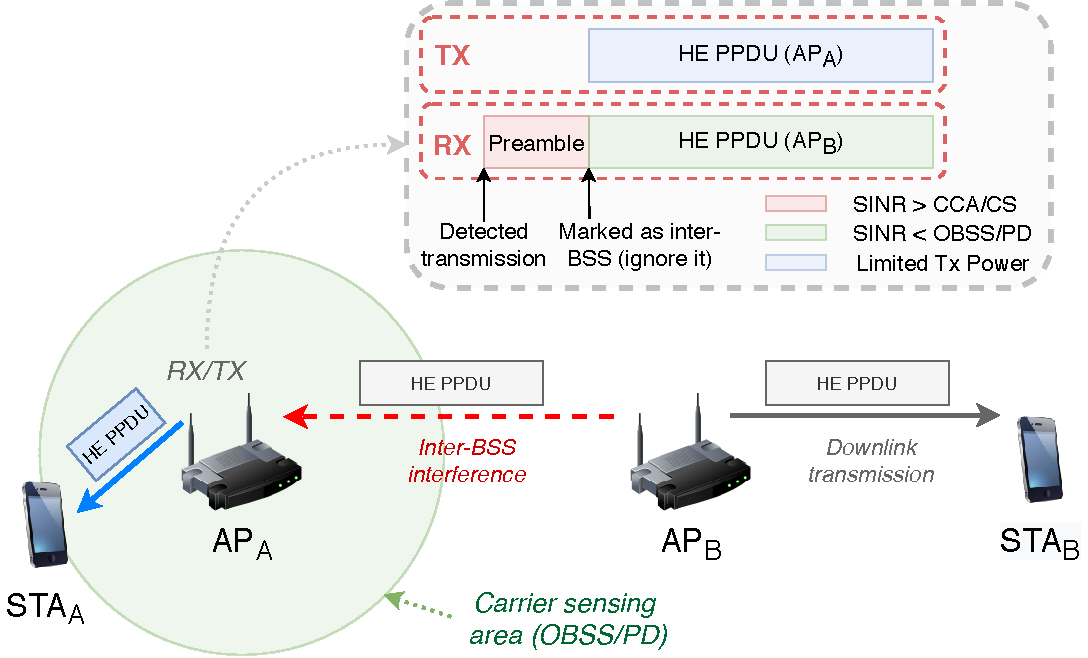
\includegraphics[width=0.8\columnwidth]{images/example_obsspd_sr}
	\caption{Example of OBSS/PD-based SR in a toy scenario.}
	\label{fig:example_obsspd_sr}
\end{figure}

% Analysis of OBSS_PD SR
The performance gains of OBSS/PD-based SR operation have been previously analyzed in \cite{mvulla2018enhanced, qu2018survey, shen2018research,malhotra2019much}.  
%\cite{malhotra2019much} evaluation of 11ax OBSS/PD-based SR.
%\cite{qu2018survey} provided some results on applying SR in both indoor and outdoor scenarios, thus showing a higher potential for indoor deployments. 
%\cite{shen2018research} provided a performance evaluation based on the adjustment of the inter-BSS sensitivity threshold. Their results showed significant gains when applying SR, especially for dense scenarios. 

% PSR 
\subsection{Parametrized Spatial Reuse}
Unlike for OBSS/PD-based SR, the PSR operation attempts to exploit triggered-based (TB) UL transmissions to carry out SR. Depending on the role of nodes participating in the PSR operation, we find two types of devices: \emph{sharing} (the ones initiating TB transmissions and indicating support for the PSR operation) and \emph{shared} (the ones taking advantage of the PSR opportunities from detected TB transmissions).

To detect PSR opportunities, shared devices must check whether their intended transmit power meets the requirements indicated in TB PPDUs from sharing devices. These requirements are based on the maximum level of interference supported by the sharing device. In particular, the minus the intended transmit power cannot exceed the following value:
\begin{equation}
\text{TX\_PWR}_{\max} = \text{TX PWR}_\text{AP} + \text{I}_\text{AP}^{\max} - RPL,
\label{eq:srp_input}
\nonumber
\end{equation}
where $\text{TX PWR}_\text{AP}$ is the normalized transmit power in dBm at the output of the antenna connector, $\text{I}_\text{AP}^{\max}$ is a normalized value in dB that captures the maximum allowed interference at the sharing device,\footnote{$\text{I}_\text{AP}^{\max}$ is computed as the target RSSI indicated in the TF minus the minimum SNR granting a 10\% PER (a safety margin is also included not to exceed 5 dB).} and Received Power Level (RPL) is measured from the legacy portion of the TF (i.e., from PHY headers).

The PSR operation is sketched in Figure \ref{fig:example_psr} for a toy scenario. As shown, the sharing device (i.e., AP$_B$) schedules an UL TB transmission by sending a TF, which is inspected by the shared device (i.e., AP$_B$) to detect a PSR-based TXOP. 
\begin{figure}[ht!]
	\centering
	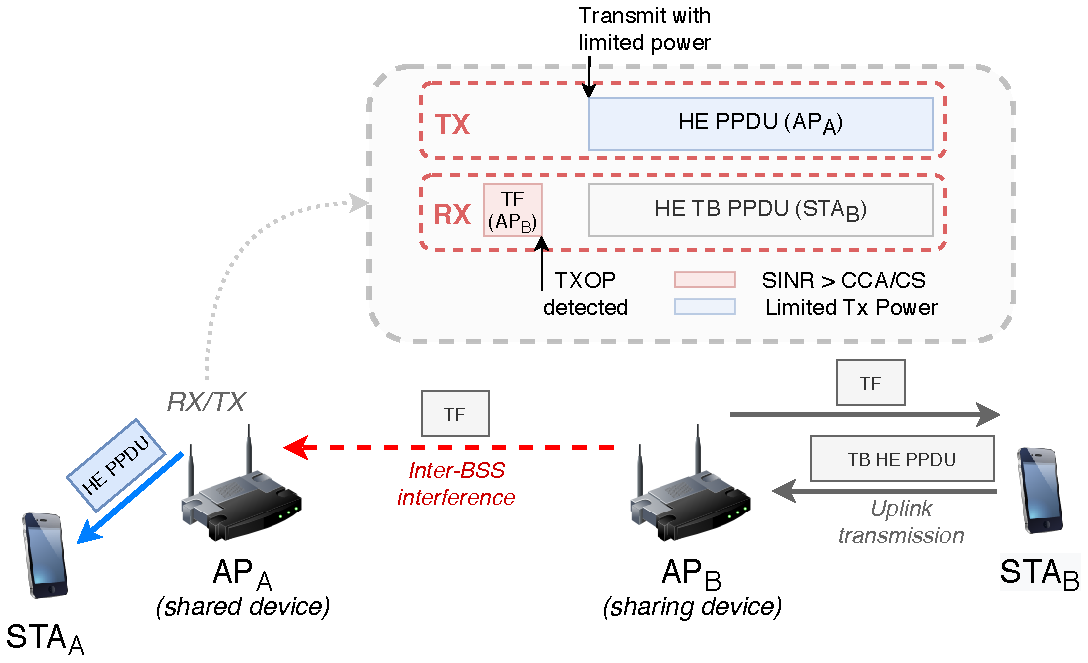
\includegraphics[width=0.8\columnwidth]{images/example_psr}
	\caption{Example of PSR in a toy scenario.}
	\label{fig:example_psr}
\end{figure}

The potential latency gains of PSR have been analyzed in \cite{carvalho2020latency}.  

% 11be and beyond
\section{Spatial Reuse in Future IEEE 802.11 WLANs}
Currently, the TGbe is studying a new coordinated scheme for SR. Notice that Multi-AP coordination (e.g., coordinated and joint transmission) is one of the main topics that has been so far been discussed by members of TGbe for coordinated beamforming (CBF)  \cite{tgbe_cbf}, coordinated OFDMA \cite{tgbe_cofdma}, and coordinated SR (CSR) \cite{tgbe_csr}.\footnote{Approved initial draft of PAR: \url{https://mentor.ieee.org/802.11/dcn/18/11-18-1231-01-0eht-eht-draft-proposed-par.docx}} 

Concerning CSR (or Co-SR), it aims to improve the quality of the simultaneous transmissions that can take place due to the SR operation. In particular, the transmit power of secondary transmissions take into account the maximum level of interference of the target devices to which transmissions are sought to be held. Co-SR is a natural extension of the SR scheme under the multi-AP operation framework and can be implemented with relatively low added complexity. 

% Other ways forward
Beyond 11be SR, the integration of SR with other novel mechanisms remains unexplored and it is expected to provide further performance gains. Among the most important techniques, we highlight beamforming/null steering \cite{tgbe_psr_beamforming}, OFDMA \cite{bankov2018ofdma, dovelos2018optimal}, multiple antenna systems \cite{liao2016mu}, and scheduled transmissions \cite{nurchis2019target}. For instance, the combination of SR with directional transmissions may lead to efficient and performance maximizing communications, where SR is applied on a per-beam basis. Similarly, SR can be further exploited through TB communications. In this case, users of a given BSS can be categorized into different types, so that different inter-BSS OBSS/PD values are assigned to them for the sake of scheduling joint transmissions. It is worth pointing out that users belonging to different groups can be scheduled together, provided that the most restrictive OBSS/PD threshold is used. 

% AI 
Finally, AI emerges as a potential solution to address SR because of the complexity of the problem and the characteristics of dense WLAN deployments, which are typically decentralized and highly varying in terms of users and channel dynamics. Through AI, it is possible to capture and exploit complex information that cannot be predicted on before-hand (traffic demands, user behavior, varying interference regimes, etc.). As a result, a learning-based procedure can be conducted to further improve the performance of WLAN deployments.

%%%%%%%%%%%%%%%%%
% MACHINE LEARNING
%%%%%%%%%%%%%%%%%
\chapter{Machine Learning in IEEE 802.11 WLANs}
\label{chapter3}

ML is meant to empower a computational system for learning automatically, based on experience, so that future situations can be properly managed without having been programmed explicitly. The actual utility of ML lies in those problems that are hard to solve by hand-programming due to their underlying complex patterns (e.g., network traffic prediction). Formally, a machine is said to learn if it improves the performance $\mathbb{P}$ obtained from undertaking task $\mathbb{T}$, based on the gathered experience $\mathbb{E}$ \cite{mitchell1997machine}. Different ML techniques have been categorized in multiple ways, but the most common taxonomy differentiates between supervised learning (labeled data is used for training), unsupervised learning (no labels are used on input data), and reinforcement learning (exploration-exploitation trade-off with label/unlabeled data).

Concerning wireless communications, the application of ML reveals a big potential because of the following aspects:
\begin{itemize}
	\item First, there is a huge amount of unexploited data generated at both infrastructure and user levels, which could be extremely useful for learning patterns that help at improving network performance.
	\item Second, current models lack of accuracy and/or tractability for capturing non-linear complex phenomena of communications systems (e.g., channel effects, varying traffic requirements, hardware imperfections, etc.). In this regard, ML does not require a mathematically tractable model to operate and can be used to address such complexities.
	\item Apart from the underlying complex characteristics of problems (e.g., wireless channel), communications systems are built based on functional blocks, each executing well defined and isolated functions (e.g., rate selection, channel allocation, etc.). While individual functions can be separately optimized, their joint operation may lead to further improve end-to-end complexity, thus hindering global optimized solutions. ML can therefore help at optimizing end-to-end processes by getting rid of the modularization of communications systems.
\end{itemize}

Henceforth, ML is expected to overcome the systemic complexity inherited from novel use cases like Vehicle to Everything (V2X) communications, Machine Type Communications (mMTC), and Ultra-Reliable Low-Latency Communication (uRLLC). In particular, the inherent flexibility of ML for automatically learning diverse situations can address heterogeneous scenarios including mobility, a huge number of devices, and varying throughput and latency requirements. For those reasons, added to the ongoing softwarization of networks, ML is expected to be pervasively included beyond the fifth-generation (5G) of mobile communications systems, namely the sixth generation (6G) \cite{calvanese2019next, shafin2020artificial, yang20196g}. Because of its high potential on addressing complex problems in communications, ML has been applied to a plethora of fields. We address the interested reader to the surveys in \cite{alsheikh2014machine, bkassiny2013survey, wang2016survey, jiang2016machine, zhang2019deep, usama2019unsupervised, klaine2017survey, cayamcela2018artificial, moysen20184g} and references therein.

\section{Computation paradigms}
Most popular ML approaches typically require a centralized architecture for training tasks on one point (e.g., a data center), which is useful for deriving global ML models encompassing data acquired from multiple sources (e.g., nodes in a network) and even from different domains (e.g., inter-operator data). This allows obtaining a general understanding of the target problem, but the accuracy of the output solution is tied to the characteristics of the training data; too diverse and complex patterns may lead to a high level of bias and model overfitting. Moreover, centralization requires certain perennity of data, thus lacking of responsiveness and not suiting real-time applications. Notice that training datasets are typically large and entail significant resource and time-consuming computational tasks. Centralized solutions are therefore very useful for problems related to the core of the network or involving higher layers of the protocols stack. For instance, DL approaches have been broadly applied for predicting periodical patterns of network traffic \cite{zhang2018long, troia2018deep, paul2019traffic} or user mobility \cite{shen2018stepdeep, zhang2020deep, li2019deep}. 

However, the access network and edge devices may face other kinds of challenges for PHY/MAC-related problems, thus requiring decentralized architectural solutions. First, end devices typically have highly-varying heterogeneous requirements and are subject to different environmental conditions. As a result, deriving a general model to properly fit all the cases can be difficult or even impossible. Second, data may fail to be integrated at a single point due to potential computation, storage or communication limitations (e.g., end devices may have low-throughput connections and be intermittently available). Third, time-consuming mechanisms requiring a heavy workload such as NNs can be barely applicable due to high non-stationarity (e.g., due to highly varying traffic demands, channel conditions, etc.), which would make trained ML models become obsolete very fast.

Decentralized approaches typically address complex and varying processes that cannot be fully learned (e.g., the learning curve is unfordable). In this regard, decentralization can provide on-time solutions rather than seeking for optimality (fast moderate improvement vs slow optimization). For that reason, techniques such as Reinforcement Learning or Sequential Learning are widely employed for PHY/MAC optimization. Some examples are resource allocation \cite{xu2017deep}, edge computing \cite{li2018deep, he2018secure}, or MIMO optimization \cite{krishnan2019optimizing}.

Figure \ref{fig:centralized_vs_decentralized} summarizes the computational approaches and implications for different problem characteristics, including requirements, available resources, and purpose.
\begin{figure}[ht!]
	\centering
	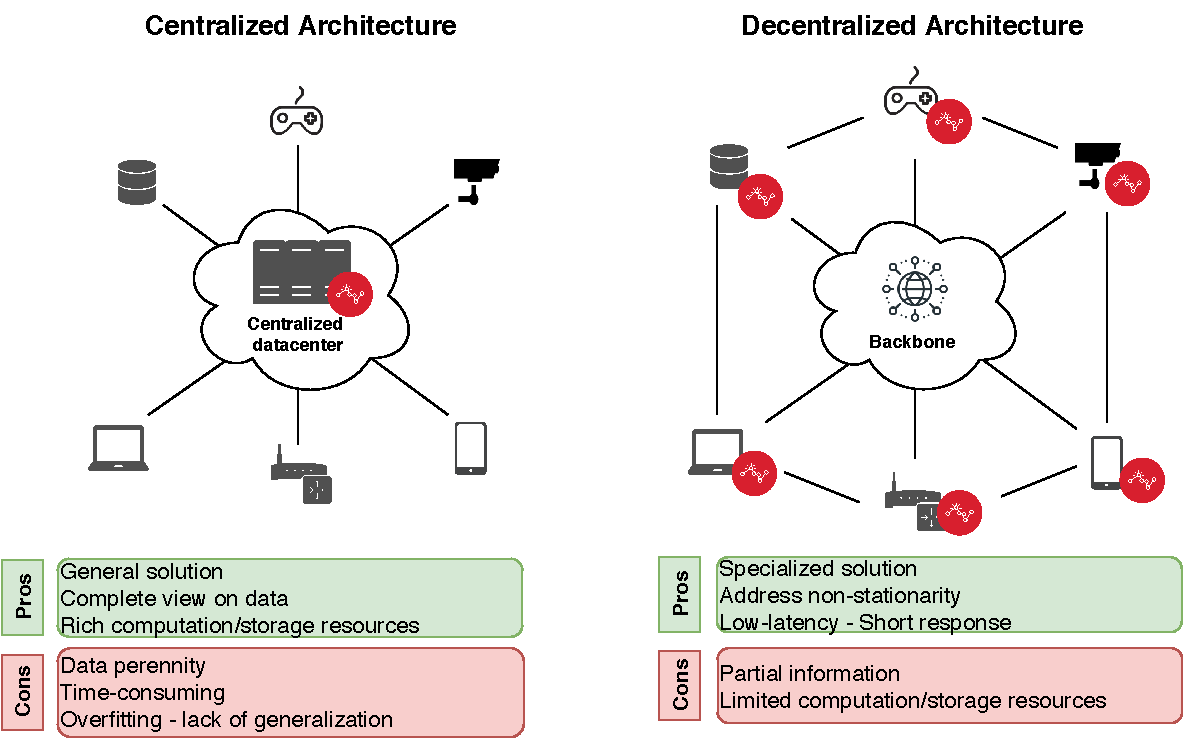
\includegraphics[width=\columnwidth]{images/centralized_vs_decentralized}
	\caption{High-level representation of centralized and decentralized architectures.}
	\label{fig:centralized_vs_decentralized}
\end{figure}

In-between centralized and decentralized systems, we find mixed architectures where other types of learning mechanisms can be applied. For instance, transfer learning (storing knowledge gained while solving one problem and applying it to a different but related problem) \cite{pan2009survey} and federated learning (collaborative training starting from a general model to better fit different contexts and situations) \cite{konevcny2016federated, smith2017federated} find a compromise that combines the power of centralized architectures and the flexibility of decentralized ones. However, the successful application of these kind of approaches is tightly tied to the communication capabilities of the implied devices, which defines the degree of cooperation among nodes in a network.

%Apart from the architectural aspects, it is important to emphasize on the way information is used: centralized, cooperative, and non-cooperative methods. Of course, the election of the approach depends on the type of problem and the set of resources available.

\section{Multi-Armed Bandits for Decentralized Spatial Reuse: Between ML and Game Theory}
The \emph{learning by experience} characteristic of sequential learning suits well to the WLANs because it allows addressing complex partial information problems. The fact is that WLANs pose a set of specific challenges resulting from their multiple deployment modes (e.g., campus network, residential usage) and their typical decentralized nature. Despite WLANs can count with plenty of data to be used by ML methods in large and planned deployments, we find other residential-type scenarios that are decentralized and lack of powerful centralized equipment. Besides, as a consequence of the abovementioned lack of coordination, a high non-stationarity is to be addressed.

\subsection{The MAB Framework}
In the MAB problem, \cite{thompson1933likelihood, bush1953stochastic}, and as for classical RL formulations, an agent (or learner) interacts with the environment to accumulate knowledge that allows responding to unforeseen events, with the aim of finding an equilibrium between exploration (improve your knowledge) and exploitation (obtain the maximum profit based on your knowledge) \cite{auer2002finite}.

% MABs formulation
Formally, a learner sequentially picks actions $a_t \in K$ and observes their reward vector $r_t$ over a time horizon $T$. Typically, the reward is granted by what is known as the environment, which may be of diverse nature (e.g., stochastic distribution, adversarial payoff). In the bandits setting, the reward follows a hidden probability distribution, and it is only revealed once the arm is played. Bandits differ from \emph{partial} and \emph{full} information settings that reveal the reward of a set or all the possible actions, respectively. 

The performance of a given action-selection strategy is typically measured by the regret $R_T$, which compares the performance achieved by the actual selected actions with the best action in hindsight granting the optimal reward ($r_t^*$). In general, an algorithm is said to learn if its regret grows sublinearly. Typical good performance is achieved for $R_T \in \mathcal{O}(\sqrt{T})$ or even $R_T \in \mathcal{O}(\log{}T)$. 

% Types of MABs and contexts of application
In spite of its simplicity, the bandits framework stands as a very powerful solution for decision making problems. The main reason lies in its versatility, which allows bandits to model almost any problem. Because of this, the utilization of bandits is nowadays widely spread, and a plethora of applications are powered by such a framework. The most typical ones are web advertising, sales optimization, online recommendations, resource allocation, and packet routing, among many others. A plethora of bandits formulations exists according to multiple assumptions that extend the basic bandits game, which are based on the reward statistics (e.g., stochastic vs non-stochastic bandits), the dynamics of actions (e.g., sleeping bandits, mortal bandits), the type of Markovian settings (e.g., rested vs restless bandits), the nature of the environment (e.g., adversarial bandits), and a very long etcetera of variations. The bandits problem has been treated in detail by several books and surveys. Table \ref{tab:bandits_categories} provides a high-level categorization of the most popular types of bandits. We encourage the interested reader to delve into the works in \cite{cesa2006prediction, gittins2011multi, bubeck2012regret, lattimore2018bandit, slivkins2019introduction}.

\begin{table}[ht!]
	\centering
	\caption{High-level categorizations of most popular bandits types.}
	\label{tab:bandits_categories}
	\begin{tabular}{|l|l|}
		\hline
		\multicolumn{1}{|c|}{\textbf{Cathegorization Criteria}} & \multicolumn{1}{c|}{\textbf{Bandits models}} \\ \hline
		Reward generation process & \begin{tabular}[c]{@{}l@{}}Stochastic, adversarial, Markovian \\ (rested/restless)\end{tabular} \\ \hline
		Reward function & \begin{tabular}[c]{@{}l@{}}Discrete, continuum (linear/nonlinear), \\ Lipschitz, Gaussian\end{tabular} \\ \hline
		Feedback type & \begin{tabular}[c]{@{}l@{}}Full information, bandit, \\ semi-bandit, partial monitoring\end{tabular} \\ \hline
		State-awareness & Multi-armed bandit, contextual bandit \\ \hline
	\end{tabular}
\end{table}

%One of the most notorious categorizations of bandits is based on the hidden model behind the reward offered by the set of available arms. In this regard, we find two main blocks, which are stochastic and non-stochastic rewards. 
%
%In stochastic bandits, the reward obtained after playing a certain action is given by a fixed probability distribution, what is to mean that every arm $k \in K$ has a fixed mean reward $\mu_k$. This assumption allows providing strong proves in terms of performance guarantees. \textcolor{blue}{Complete this part with typical regret bounds (upper and lower).} When it comes to non-stochastic bandits, the previous assumptions do not hold since ...

\subsection{MAB in Communications}

In wireless communications, many problems have statistical characteristics that can be approximated with mathematical models. In this regard, MAB-based applications have shown a great potential for optimizing a plethora of problems. Some examples are channel selection \cite{gai2010learning}, spectrum access \cite{tekin2011online}, transmission scheduling \cite{chen2006transmission}, or AP selection \cite{carrascosa2019decentralized}. Table \ref{tab:mabs_communications} provides an overview of some popular applications in communications that are based on the MABs framework.

\begin{table}[]
	\caption{Overview of bandit-based applications for communications}
	\label{tab:mabs_communications}
	\resizebox{\textwidth}{!}{%
		\begin{tabular}{|l|l|l|l|l|}
			\hline
			\multicolumn{1}{|c|}{\textbf{Problem}} & \multicolumn{1}{c|}{\textbf{Modeling}} & \multicolumn{1}{c|}{\textbf{Goals}} & \multicolumn{1}{c|}{\textbf{\begin{tabular}[c]{@{}c@{}}Baseline \\ algorithms\end{tabular}}} & \multicolumn{1}{c|}{\textbf{References}} \\ \hline
			\begin{tabular}[c]{@{}l@{}}Opportunistic \\ spectrum access \& \\ Channel selection\end{tabular} & \begin{tabular}[c]{@{}l@{}}Stochastic, non-stochastic, \\ restless, contextual, Markovian\\ bandits\end{tabular} & \begin{tabular}[c]{@{}l@{}}Decentralized optimal allocation, \\ optimize number of secondary\\ transmissions, $\epsilon$-correct ranking\end{tabular} & \begin{tabular}[c]{@{}l@{}}UCB, $\epsilon$-greedy,\\ calibrated forecasting\end{tabular} & \cite{liu2008restless,gai2010learning, tekin2011online,anandkumar2011distributed,rosenski2016multi,maghsudi2015channel} \\ \hline
			Power control & Non-stochastic bandits & Optimize SINR & \begin{tabular}[c]{@{}l@{}}Follow the perturbed leader,\\ exponential weighted average\end{tabular} & \cite{maghsudi2014joint} \\ \hline
			User association & \begin{tabular}[c]{@{}l@{}}Sleeping, Bernoulli,\\ non-stochastic bandits\end{tabular} & Energy saving, improve the throughput & UCB, $\epsilon$-greedy & \cite{maghsudi2017distributed,carrascosa2020multi} \\ \hline
			Inter-cell coordination & \begin{tabular}[c]{@{}l@{}}Adversarial, stochastic,\\ non-stochastic,\\ contextual bandits\end{tabular} & \begin{tabular}[c]{@{}l@{}}Optimize inter-cell frequency resources,\\ energy saving, map SON configurations \\ and operator objectives\end{tabular} & EXP3, UCB, $\epsilon$-greedy & \cite{coucheney2015multi, feki2011autonomous, ayala2018contextual, daher2017cognitive} \\ \hline
			Dynamic rate selection & Structured, Markovian bandits & \begin{tabular}[c]{@{}l@{}}Maximize the number of packets \\ successfully transmitted, \\ learn changes in the channel\end{tabular} & UCB & \cite{combes2014dynamic, zhao2020non} \\ \hline
			LTE/Wi-Fi coexistence & Convex bandits & Fair channel sharing & Online gradient descent & \cite{cano2018wireless} \\ \hline
		\end{tabular}%
	}
\end{table}

% Nexus with Game Theory and why equilibrium can be reached
Concerning the decentralized SR problem, it can be naturally defined as a multi-agent system, where each individual (e.g., a BSS) has player-specific goals and rewards.\footnote{The maximum achievable performance of a node depends on its transmission capabilities, the interference it senses, the traffic load it needs to serve and/or receive, etc.}  The multi-agent approach allows capturing the distributed nature of IEEE 802.11 WLANs and keeping dimensionality low for the SR problem. However, it may unleash a competition among players, thus revealing a nexus with game theory. In a single-agent system, a player attempts to maximize a long-term reward by interacting with an environment (which can be stochastic or non-stochastic) in isolation. Under this setting, performance guarantees can be straightforwardly provided, even if dealing with adversarial \cite{auer2002nonstochastic} or dynamic environments \cite{gupta2011thompson}. In contrast, weaker performance guarantees can be provided for multi-agent systems. The fact is that knowledge acquired by agents becomes easily outdated because of the non-stationarity produced by their concurrent operation.

Most of the current literature in multi-player MABs for wireless communications is based on the channel access problem in cognitive radio \cite{gai2010learning, liu2008restless, anandkumar2011distributed, di2011learning, bkassiny2013survey, cohen2014restless, abbas2015recent, maghsudi2015joint, avner2014concurrent}. The characteristics of the cognitive radio make it a suitable and an attractive problem to be modeled with the bandits framework. In particular, each node attempting to access the channel represents a player, and channels are arms (or bandits). In general, rewards are granted to players in a binary fashion, being 1 if the channel can successfully be accessed, or 0 otherwise (two or more nodes select the same channel). Accordingly, each player has the same view on actions (different players playing the same bandit obtain to the same payoff), which makes the game smooth, i.e., the reward function of the players is continuous with respect to the entire strategy set. Table \ref{tab:mpmab_cr} analyzes the state-of-the-art approaches taken for modeling channel access in cognitive radio through multi-player MABs.

\begin{table}[]
	\caption{State-of-the-art multi-player MAB solutions for channel access in cognitive radio.}
	\label{tab:mpmab_cr}
	\resizebox{\textwidth}{!}{%
		\begin{tabular}{|c|l|l|l|}
			\hline
			\textbf{Work} & \multicolumn{1}{c|}{\textbf{Approach}} & \multicolumn{1}{c|}{\textbf{Requirements}} & \multicolumn{1}{c|}{\textbf{Results}} \\ \hline
			\cite{anandkumar2011distributed} & \begin{tabular}[c]{@{}l@{}}Distributed mechanism that \\ combines sensing with randomized \\ access to learn channel statistics \\ and the activity of other users\end{tabular} & \begin{tabular}[c]{@{}l@{}}- The number of users is fixed and known\\ - Channel sensing is perfect\\ - All the players use the same strategy\\ - Binary reward (free/collision)\end{tabular} & \begin{tabular}[c]{@{}l@{}}Order-optimal regret with \\ logarithmic lower bound\end{tabular} \\ \hline
			\cite{liu2010distributed} & \begin{tabular}[c]{@{}l@{}}Decentralized time-division fair \\ sharing of the best arms\end{tabular} & \begin{tabular}[c]{@{}l@{}}- i.i.d. reward\\ - Conditions of linearity, continuity, \\ and density for unknown parameters\\ - Binary reward (free/collision)\\ - The number of users is fixed and known\end{tabular} & \begin{tabular}[c]{@{}l@{}}Same logarithmic regret order \\ as for collaborative approach \\ where nodes exchange observations \\ and make decisions jointly\end{tabular} \\ \hline
			\cite{di2011learning} & \begin{tabular}[c]{@{}l@{}}Collaborative mechanism based on\\ slotted periods (decision, sensing,\\ transmission, communication)\end{tabular} & \begin{tabular}[c]{@{}l@{}}- Channel sensing is done\\ - CSMA/CA is used by secondary users\\ - Rewards are broadcasted\\ - Same channel conditions for all users\end{tabular} & \begin{tabular}[c]{@{}l@{}}Linear regret improving random\\ and greedy channel access schemes\end{tabular} \\ \hline
			\cite{maghsudi2015channel} & \begin{tabular}[c]{@{}l@{}}Distributed no-regret learning with\\ calibrated forecaster\end{tabular} & \begin{tabular}[c]{@{}l@{}}- The joint action profile is known\\ - All the players use the same strategy\\ - Time-invariant average channel gains\end{tabular} & \begin{tabular}[c]{@{}l@{}}Global optimal solution and \\ convergence to correlated equilibria\end{tabular} \\ \hline
			\cite{avner2014concurrent} & \begin{tabular}[c]{@{}l@{}}Non-cooperative selfish approach\\ based on $\epsilon$-greedy exploration \\ and CSMA/CA\end{tabular} & \begin{tabular}[c]{@{}l@{}}- K $\geq$ N ($K$: channels, $N$: users)\\ - The number of users is fixed and known\end{tabular} & \begin{tabular}[c]{@{}l@{}}Sub-linear regret and convergence to \\ system-optimal solution\end{tabular} \\ \hline
			\cite{gai2010learning} & \begin{tabular}[c]{@{}l@{}}Centralized method for combinatorial\\ bandits with user-channel pairs\end{tabular} & \begin{tabular}[c]{@{}l@{}}- K $\geq$ N ($K$: channels, $N$: users)\\ - Throughput as an i.i.d. random variable\\ - Coordination/synchronization\end{tabular} & \begin{tabular}[c]{@{}l@{}}Upper bound regret that grows \\ polynomially with the combinatorial \\ number of users and channels\end{tabular} \\ \hline
		\end{tabular}%
	}
\end{table}

\subsection{MAB-based Decentralized Spatial Reuse}

In the MABs setting, optimal solutions can typically be provided only to tractable problems that are generally linear, stationary, and generated by independent stochastic processes (e.g., with underlying Gaussian statistics). This is not the case of the multi-agent SR problem, in which it is not possible to provide a distributed no-regret strategy that converges to an optimal equilibrium. The fact is that the set of correlated equilibria cannot be characterized in the SR problem with multiple concurrent players. In particular, the following properties differing from distributed channel access prevent to do so:
\begin{enumerate}
	\item Spatial interactions inflict abrupt changes to the reward obtained by a BSS, which can be based, for instance, on the throughput. To put an example, increasing the sensitivity contributes to reducing contention, but it may lead to noticing a higher amount of interference during transmissions. 
	\item Apart from spatial interactions, devices do not transmit uniformly along the time, which is in fact an unrealistic assumption. Therefore, the social-cost of actions varies with time and according to the transmissions done on a per-packet-basis (where certain randomness is added due to many causes such as channel effects, retransmissions, the randomized backoff procedure, etc.).
\end{enumerate}

In these situations, defining a shared learning goal in multi-agent systems is not trivial because rewards are not equally assigned to agents and each individual reward depends on the joint action profile. Nonetheless, MABs remain a powerful solution to address real-world problems with complex and even unpredictable phenomena behind reward distributions. This is the case of the multi-player setting (i.e., multiple agents attempt to learn concurrently), which entails the enormous challenge of non-stationary, but for which on-time improvements prevail over long-term optimality. 

In the following subsections, we show the different settings that have been considered for applying concurrent SR through MABs, which are based on the cooperation degree among BSSs (selfish, collaborative, and social-aware). In cooperative scenarios, agents collaborate to optimize a common goal (e.g., a shared reward), which is attempted to be maximized jointly. When it comes to non-cooperative approaches, local rewards are employed to characterize selfish behaviors, i.e., each agent attempts to improve its own performance. 

\subsubsection{Selfish Setting}
\textcolor{red}{[TBD]} \textcolor{red}{Idea: formulate the problem and devise implications and opportunities.}

\textit{Under the selfish setting, several concurrent agents attempt to improve their own performance, based on local information. In the case of SR, actions are defined as combinations of sensitivity and transmit power values.}

\textit{While the selfish setting has been shown to provide fast learning rates \cite{wilhelmi2019collaborative}, it may also provoke several undesired issues such as sub-optimal performance and unfairness \cite{wilhelmi2019potential}. Nevertheless, a collaborative behavior was shown to be achieved, thus leading to an equilibrium.}

\subsubsection{Collaborative Setting}
\textcolor{red}{[TBD]} \textcolor{red}{Idea: formulate the problem and devise implications and opportunities.}

\textit{In this case, an environment-aware strategy is provided for deciding the best transmit power and sensitivity configuration, based on the performance of the overlapping networks into account. Despite a fair solution is shown to be achieved, certain limitations were revealed for maximizing the overall performance, thus showing that a shared reward is not enough in a decentralized setting.}

\subsubsection{Social-Aware Setting}
\textcolor{red}{[TBD]} \textcolor{red}{Idea: formulate the problem and devise implications and opportunities.}

\textit{To overcome the issues raised by both selfish and shared reward settings, we focus on hybrid approaches by considering a social-aware cost function, which combines both local and collaborative rewards. In this regard, we highlight the work in \cite{maghsudi2015joint}, which includes transmission power control to the distributed channel access problem in cognitive networks. Given a proposed model for opportunistic spectrum access, the authors are able to provide distributed no-regret strategies that lead to the set of correlated equilibria. However, some assumptions are made to provide convergence guarantees. In particular, the reward function used by the players is continuous with respect to the strategy set, which is also bounded. Intuitively, this means that the social cost that any action incurs to the other players can be linearly quantified. }

%%%%%%%%%%%%%%%%%
% METHODS
%%%%%%%%%%%%%%%%%
\chapter{Methodology and Enablers} 
\label{chapter4}
\textcolor{red}{[TBD]}
% CTMNs model
\section{Spatial Reuse through Continuous Time Markov Networks}
Characterizing the IEEE 802.11ax SR operation is crucial to fully understand its implications. However, it turns out to be a challenging task due to the complex (and still unknown) inter-WLAN interactions generated by adjusting the sensitivity and the transmission power. To the best of our knowledge, none of the previous works have attempted to model the 11ax SR operation. Nevertheless, with the aim of providing a thorough understanding of the SR operation, we introduce the CSMA/CA throughput model based on Continuous Time Markov Networks (CTMNs) \cite{bellalta2014throughput,bellalta2017throughput}. The CTMNs model aims to provide further insight into the effects of applying SR in next-generation WLANs.

The CTMN model captures the CSMA/CA operation used in IEEE 802.11 WLANs
through states, which represent the set of WLANs that are active at a given moment. Transitions between states occur when WLANs become active (i.e., they gain access to the medium) or when they abandon the channel (i.e., their transmission is finished).

Analyzing inter-BSS MAC interactions is of great utility to deeply understand the implications of applying SR in WLANs. For that, we have modeled SR through Continuous Time Markov Networks (CTMN) \cite{bellalta2014throughput,bellalta2017throughput}, based on the framework presented in \cite{barrachina2019dynamic}.\footnote{The SFCTMN framework has been extended for the SR operation in \url{https://github.com/sergiobarra/SFCTMN/tree/single_channel_IEEE80211ax_spatial_reuse}} Concerning this model, the following assumptions are done:
\begin{itemize}
	\item Transmissions are downlink only.
	\item Uplink transmissions of control packets (e.g., ACKs) are only considered to compute the total transmission time. This implies that we do not consider uplink transmissions for modeling inter-BSS interactions.
	%
\end{itemize}

First, the backoff procedure for accessing the medium is continuous in time. Thus, collisions due to backoff expiring at the same
instant are not captured by the model. Second, downlink traffic is considered. Accordingly, the model is focused on finding inter-AP interactions.
It is important to highlight that additive interference is considered, which results from the combination of different simultaneous
interfering transmissions. Accordingly, we are able to characterize real deployments where spatially-distributed interactions occur. Moreover, traffic is considered to be saturated in all the nodes, so that pure SR-based interactions become more apparent.

% 11ax OBSS/PD-based SR
\subsection{IEEE 802.11ax OBSS/PD-based Spatial Reuse}

In order to model the 11ax SR operation, we have considered the generation of new states,
which are related to the different sensitivity levels that each WLAN can use. Notice that
using different sensitivity levels enables, on the one hand, to find new types of inter-WLAN
interactions that could not exist without applying SR. On the other hand, increasing the
sensitivity entails decreasing the transmission power. As a result, the capabilities of a given
node vary according to the OBSS/PD threshold that is employed in every situation; a lower
transmission power entails using a more robust Modulation and Coding Scheme (MCS).

% 11be CSR
\subsection{IEEE 802.11be Coordinated Spatial Reuse}

%	\item Coordinated transmissions will always have priority if they are possible. For instance, if we have two coordinated BSSs (A and B) that can transmit simultaneously, the joint transmission will occur over individual ones (e.g., if A wins contention, the transmission will be in coordination with B, rather than transmitting A only). 
%	%
%	\item The feasibility of a coordinated transmission is only assessed from the perspective of the sharing AP. This means that we do not consider if the transmission of the shared AP will fail or succeed. 
%	%
%	\item Sharing and shared transmission duration are equal.

% Simulation
\section{System-level Simulation of Spatial Reuse}
In addition to the analytical model, we introduce the 11ax SR operation in the Komondor simulator. This simulator was conceived, among other purposes, to allow the low-cost integration of novel mechanisms included in new IEEE 802.11 standards. This is the case of the 11ax SR operation, which has not been yet fully implemented in any other well-known simulator. To the date of publishing this article, SR is still being developed for ns-3. By comparing our simulation results with the analytical model, we expect to shed some light on the effects of using 11ax SR, particularly with regard to inter-WLAN interactions. The analytical model will assist us in drawing conclusions regarding the network dynamics that can occur when applying the SR operation.

% Architecture
\section{Architectural Aspects of Machine-Learning-Aware Networks}

Finally, we delve into the architectural aspects for enabling ML-aware networking solutions. The fact is that the existing infrastructure is not yet prepared to accommodate ML-oriented tasks such as data collection, processing, and output distribution. Instead, current networking systems are typically meant for delivering content, without taking into account the underlying characteristics of the processes that generate it.

The first steps towards AI-enabled networking are currently being made in 5G through Network Function Virtualization (NFV). Unlike traditional hardware-based networks, NFV allows rapid elasticity and fast reconfiguration on assigning network resources. This is particularly useful to enable verticals such as autonomous driving in the automotive sector or smart manufacturing in industry 4.0. Besides, network virtualization is useful to boost inter-operator coordination and bringing the ML operation to a macro-scale level, counting with vast information and computation resources. 

To conduct the evolution towards ML-aware networks, standardization is key to reach consensus between operators and manufacturers. In this regard, we find many initiatives held by standardization organizations, from which we highlight the Focus Group on Machine Learning for Future Networks including 5G (FG-ML5G), which belongs to the International Telecommunication Union Telecommunication Standardization Sector (ITU-T). The FG-ML5G aims to enable the convergence of future communications with ML technologies. To that end, the focus group has released a specification on a \emph{Unified architecture for 5G and beyond}, recently turned into an ITU Recommendation \cite{itu2019architecture}. Remarkably, ITU's standardized architecture provides a common nomenclature for ML-related mechanisms so that interoperability with other networking systems is achieved. 

The module-based ITU's architecture allows adapting  to  the problem  instance  and  the  set  of  available  resources,  thus providing flexibility in terms of deployment heterogeneity. For instance, despite deep learning is a powerful solution that may improve  the  performance  in  multiple  scenarios,  it  entails a set of computation, storage and communication requirements that may not be fulfilled in other deployments, or parts of the network

%Federated learning: The system then needs to communicate and aggregate the model updates in a secure, efficient, scalable, and fault-tolerant way. It's only the combination of research with this infrastructure that makes the benefits of Federated Learning possible.

Apart from the ITU-T initiatives, other important standardization bodies such as the 3rd Generation Partnership Project (3GPP) or the European Telecommunications Standards Institute (ETSI) are currently working on the integration of data analytics to network functions. The 3GPP contemplates AI as one of the priority topics for shaping its upcoming release (Release 17) and architectural requirements are currently under study \cite{3gpp2019study}. Furthermore, we highlight the ETSI groups on Experiential Networked Intelligence (ENI) and Zero-touch network and Service Management (ZSM), which actively study the integration of AI to networks \cite{etsi2019architecture}. Unlike the ITU's unified architecture, most of the work held by the 3GPP and the ETSI focuses on centralized data collection and data analytics solutions. Nevertheless, we understand that the works in \cite{itu2019architecture, 3gpp2019study, etsi2019architecture} are complementary to each other.


% 1 - Architectural proposals	
Apart from the specific ML solutions to problems in communications, some efforts have been made towards enabling AI-aware networking in more general terms. In particular, several architectural proposals have been provided so far \cite{bi2015wireless,chih2017big,wang2018machine}. Most of the referenced works agree in the necessary steps for enabling big data analytics in cellular deployments: (1) data collection, (2) data preparation, (3) data analysis, and (4) decision making. Nevertheless, none of these works provide architectural guidelines to introduce ML to wireless networks. In this regard, the ITU's architecture looks deeper into the ML operation and targets the actual procedures involving information gathering, processing, and communication. Besides, the ITU-T provides a data handling framework for ML-aware networks \cite{itu2019data}, which defines processes concerning data collection, processing, and output distribution.

%%%%%%%%%%%%%%%%%
% RESULTS
%%%%%%%%%%%%%%%%%
\chapter{Main Findings}
\label{chapter5}

\textcolor{red}{[TBD]}

%%%%%%%%%%%%%%%%%
% CONCLUSIONS
%%%%%%%%%%%%%%%%%
\chapter{Open Challenges and Future Work}
\label{chapter6}

\textcolor{red}{[TBD]}

%%%%%%%%%%%%%%%%%
% BIBLIOGRAPHY
%%%%%%%%%%%%%%%%%
\bibliography{bibliography}

%%%%%%%%%%%%%%%%%
% ATTACHED PUBLICATIONS
%%%%%%%%%%%%%%%%%
\chapter{Publications}
\label{chapter7}

\section{Spatial Reuse in IEEE 802.11 ax WLANs}

\section{On the Performance of the Spatial Reuse Operation in IEEE 802.11 ax WLANs}

\section{Implications of decentralized Q-learning resource allocation in wireless networks}

\section{Collaborative spatial reuse in wireless networks via selfish multi-armed bandits}

\section{Potential and pitfalls of multi-armed bandits for decentralized spatial reuse in WLANs}

\section{A Flexible Machine-Learning-Aware Architecture for Future WLANs. IEEE Communications Magazine}

\section{Komondor: a wireless network simulator for next-generation high-density WLANs}

\section{Usage of Network Simulators in Machine-Learning-Assisted 5G/6G Networks}

\backmatter
\printindex

\end{document}

%NUMBER OF THE EXTERNAL PAGE EXCEPT IN THE FIRST PAGE OF EACH CAPITAL
\usepackage{fancyhdr}
\pagestyle{fancy}
\fancyfoot{}
\fancyfoot[RO]{\thepage}
\fancyfoot[LE]{\thepage}

%MULTIPLE INDEX
%In the preamble
\usepackage{multind}
\makeindex{authors}
%Introduction to form entries
\index{authors}{Einstein}
%Situation of the Index
\printindex{authors}{Author index}
%The \ usepakage {makeidx} \ makeindex \ printindex commands must be removed
%You need to exacute from the command line makeindex authors